\section{Introduction}
\label{sec:introduction}

\paragraph{From Single-Pass Rendering to Closed-Loop Visual Creation.}
Visual generation has developed from a specialized media-synthesis capability into a general component of artificial intelligence infrastructure. It now supports the production and editing of images, videos, three-dimensional assets, data-grounded graphics, structured documents, interactive interfaces, and related visual artifacts across design, entertainment, education, science, industry, and other application settings. Advances in generative and multimodal models have substantially improved visual fidelity, instruction and reference adherence, text rendering, controllability, editing, and other task-specific capabilities \cite{he2024llms,yang2025textimage,wang2025imageediting,yin2025spatiotemporal}. A single-pass renderer can now often produce a plausible artifact from a concise instruction and a limited set of conditions.

% P7 (optional): place a schematic figure here contrasting an open-loop
% single-pass pipeline (errors accumulate downstream) with a closed loop
% (O -> pi -> U, with the observation arrow feeding back into action choice)
% to anchor the survey's central contrast visually.

The expansion from isolated synthesis to multi-step visual creation tasks changes the requirements placed on a visual system. A single artifact or sequence may need to preserve precise spatial relations, target identity, temporal order, editable structure, factual or data-grounded content, physical plausibility, stable interaction, and other cross-step requirements. Surveys, benchmarks, and recent system studies continue to report weaknesses along structural, temporal, physical, and other task-specific dimensions even when individual outputs achieve high perceptual quality \cite{wu2026visualgeneration,yin2025spatiotemporal,avg250925229,feng2026newton}. Their practical consequence is cumulative: an early relation error can invalidate a later edit, identity drift can propagate through a video, an incorrect data mapping can undermine a scientific graphic, and an invalid geometric operation can make a visually plausible model unusable, among other downstream effects. Meeting these requirements calls for creation control: constraint persistence, usable intermediate state, diagnosis, repair, and other forms of trajectory management.

Model scaling, prompt refinement, additional conditioning, repeated sampling, and other output-level refinements can improve individual outputs. None of them closes the loop: a visual creation process remains open-loop when runtime observations do not change subsequent decisions. Under this condition, the system cannot use intermediate outcomes to determine whether the current plan remains appropriate, which constraints have been satisfied or violated, where a failure has occurred, or when the task should stop. Local errors and changes in task state may then persist or propagate across later edits, frames, components, and other dependent outputs.

Avoiding such accumulation requires goal-directed control over the creation trajectory. The system must maintain task-relevant state, inspect intermediate artifacts and execution outcomes, and use the resulting evidence to determine subsequent actions. Recent years show rapid progress toward this capability: since 2024, systems combining artifact observation, constraint verification, tool selection, and iterative correction have emerged across compositional image generation \cite{wang2024divide}, programmatic video production \cite{he2024kubrick}, and multi-turn image editing \cite{gupta2025costa}, with early extensions toward physical generation, scientific visualization, and structured documents. These developments mark a transition from open-loop sampling toward closed-loop visual creation, in which runtime observations change later action selection.

% NOTE: if the template is double-column, change \begin{figure} to \begin{figure*}
\begin{figure}[t]
  \centering
  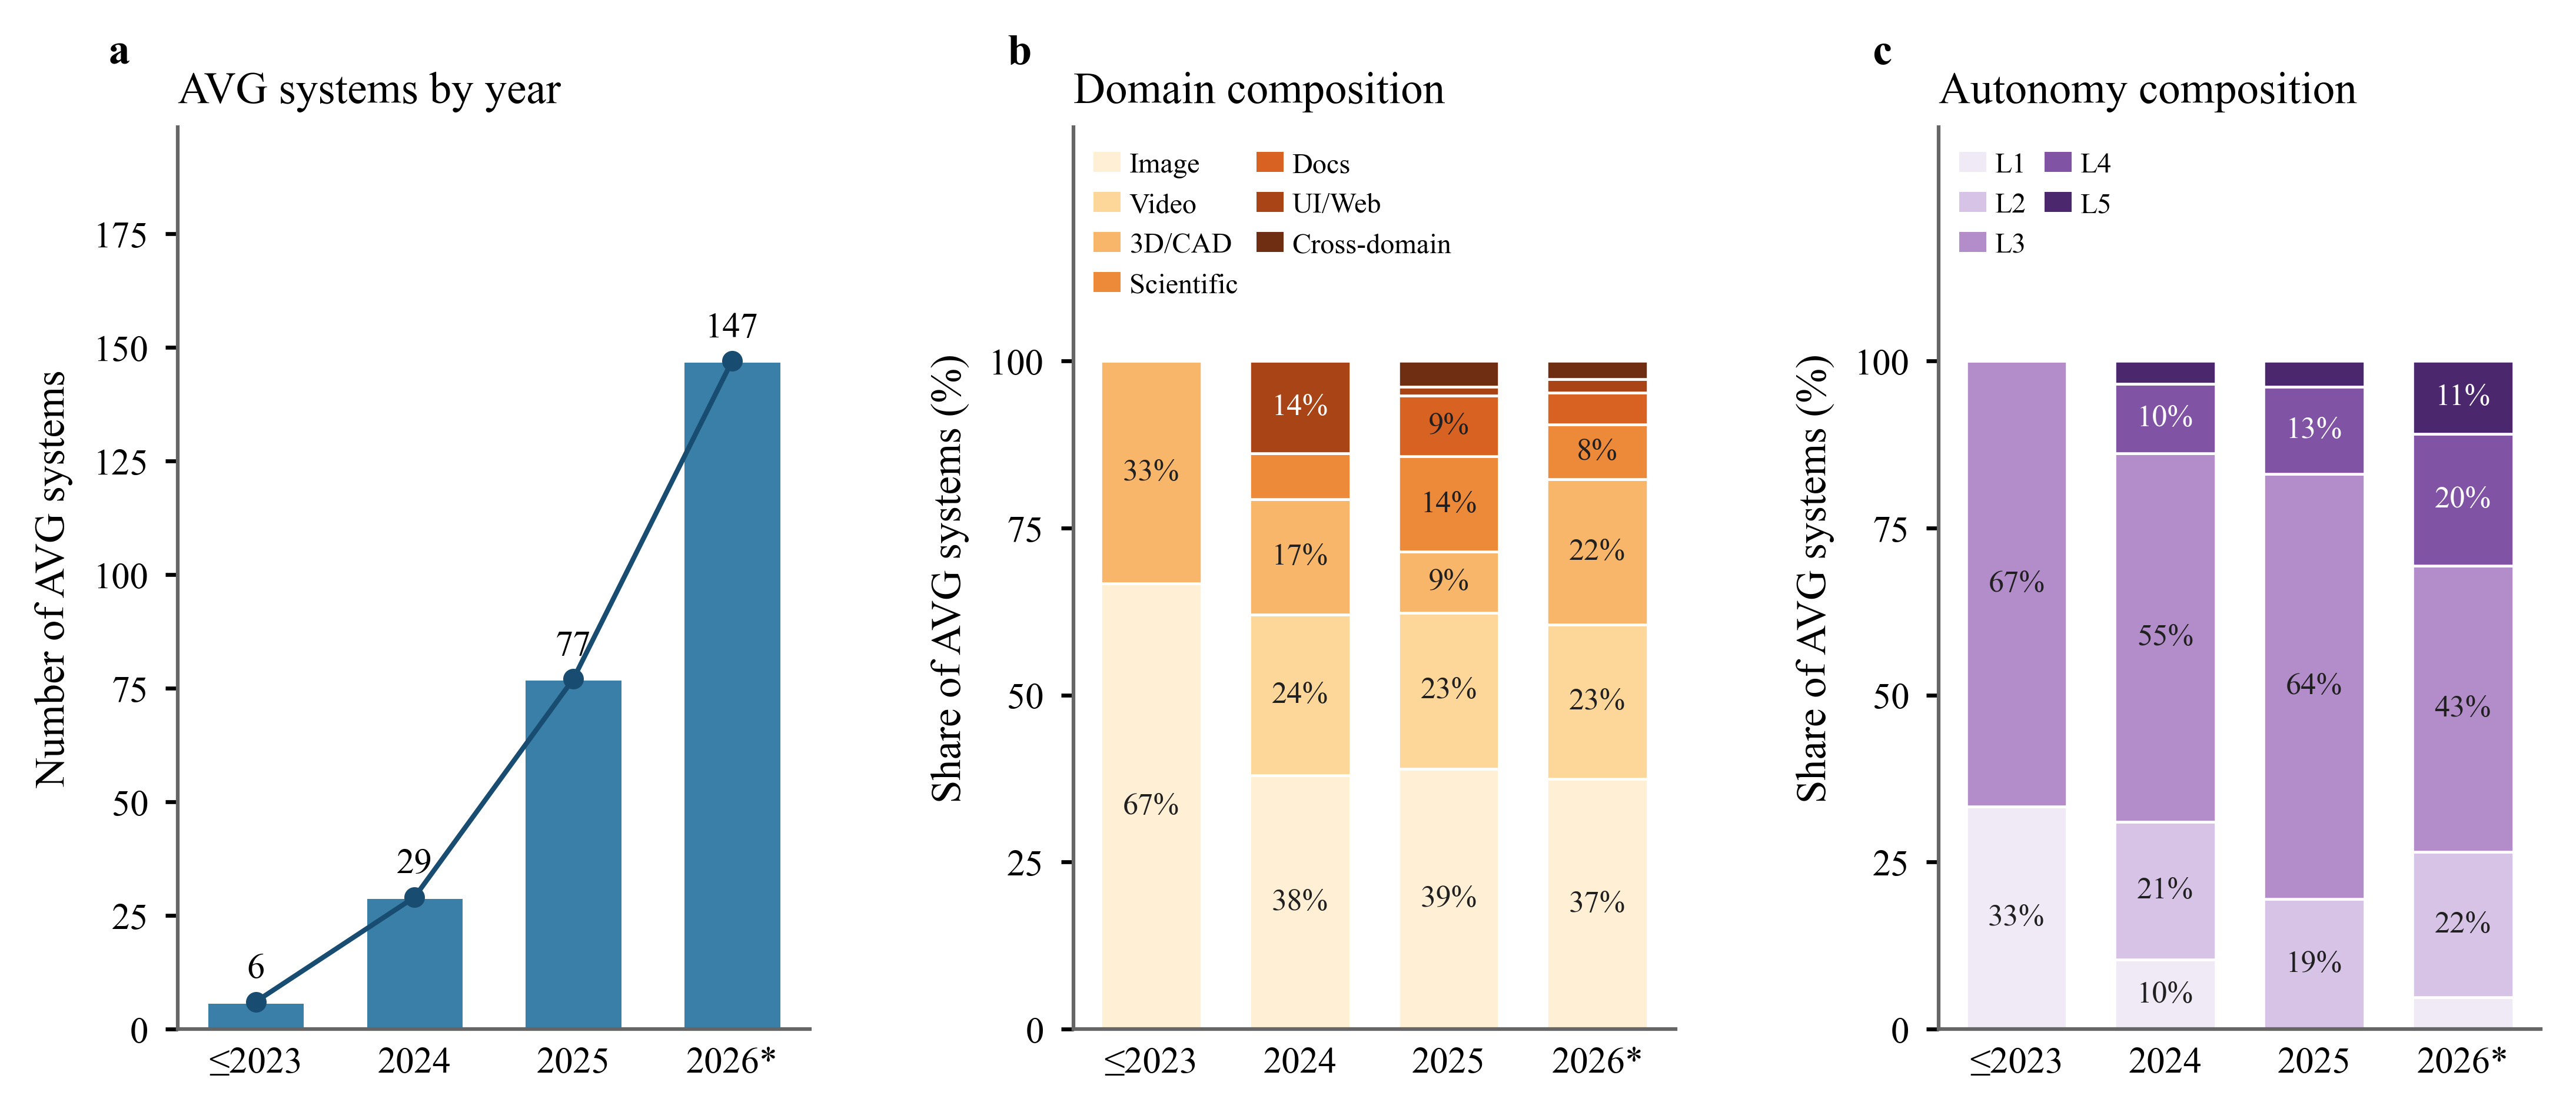
\includegraphics[width=\textwidth]
    {figures/avg_literature_growth_by_year_domain_autonomy.jpg}
  \caption{Growth and composition of the surveyed literature on agentic
  visual generation. \textbf{a}, Number of included systems grouped by
  first arXiv year, with records up to 2023 pooled. \textbf{b}, Visual-domain
  composition within each period. \textbf{c}, Composition by the highest
  autonomy level supported by the reported evidence. The asterisk marks
  partial-year coverage for 2026 at the dataset cutoff. Counts reflect the
  survey corpus and coding protocol rather than all publications on visual
  generation.}
  \label{fig:avg-literature-growth}
\end{figure}

Figure~\ref{fig:avg-literature-growth} quantifies this transition across the surveyed corpus; the inclusion criteria and coding protocol are described in Section~\ref{sec:foundations}. The number of systems expands rapidly after 2023 (panel~a), and the growth spans visual domains: closed-loop designs now appear across images, video, three-dimensional assets, data-grounded graphics and documents, and interactive interfaces (panel~b), so the same control questions recur under different representations, constraints, and sources of verification evidence. The composition by autonomy level shifts upward in parallel, with a growing share of systems reporting behaviors beyond fixed pipelines (panel~c), as graded by the L1--L5 levels introduced in Section~\ref{sec:foundations}. Yet the aggregate trend also exposes the gap behind the growth: the designs remain scattered across application papers, autonomy claims rest on heterogeneous evidence, and no unified, control-centered account exists of what makes such systems agentic, how they should be organized, or how they should be evaluated.

In this survey, we develop that account. We name this class of systems \emph{agentic visual generation} (AVG) and present its working definition below.

\begin{keytakeawaytight}[Working Definition of AVG]
\emph{Agentic visual generation} is goal-driven visual creation organized as a closed loop over a multi-step trajectory. At the decision points exposed to the controller, such as which operation or tool to invoke, which repair target to address, and whether to continue or stop, the system selects among available alternatives based on runtime observations. These observations are drawn from accessible, task-relevant state spanning the evolving visual artifact, its task environment, and the interaction history, which is in turn updated by intermediate artifacts, execution outcomes, external information, user feedback, and other task-relevant sources. The defining behavioral property is therefore a demonstrable observation--action dependency: runtime observations change later action selection.
\end{keytakeawaytight}


\paragraph{Review Motivation and Questions.}
Existing related surveys examine adjacent questions from different starting points. Visual-generation surveys organize the literature around model families, conditioning and editing methods, or particular visual tasks and modalities \cite{yang2025textimage,wang2025imageediting,yin2025spatiotemporal}. The survey of He et al.\ studies how language models participate in multimodal generation and editing, including through tool-mediated interaction \cite{he2024llms}. Agent surveys instead develop concepts, capabilities, and system designs for language agents or multimodal agents across broad task settings \cite{durante2024agentai,xie2024large,jiang2024rationality,schneider2025generative}. At a different level of abstraction, the recent visual-generation roadmap situates agentic generation within a longer progression toward visual intelligence and world modeling \cite{wu2026visualgeneration}.

These reviews provide essential foundations, but their primary questions differ from the one considered here. To the best of our knowledge, no existing survey is devoted specifically to agentic visual generation as a class of systems in which runtime observations demonstrably change subsequent visual-creation decisions. This survey uses that behavioral property to organize the literature, then compares how the resulting control mechanisms and supporting evidence vary across visual-creation domains.

The survey addresses six research questions:

\begin{enumerate}
  \item \textbf{Conceptual boundary:} What constitutes AVG, and how does it relate to one-shot generators, fixed workflows, and agent-augmented workflows? (Section~\ref{sec:foundations})
  \item \textbf{Analytical components:} Which components organize the connection between runtime observations and subsequent visual-creation decisions? (Section~\ref{sec:components})
  \item \textbf{Cross-domain variation:} How are these mechanisms realized across visual-creation domains? (Sections~\ref{sec:image-generation}--\ref{sec:cross-domain})
  \item \textbf{Training and improvement:} How are AVG systems trained and improved through trainable components, visual trajectories, feedback, experience reuse, and cross-task transfer? (Section~\ref{sec:training})
  \item \textbf{Evaluation:} How should the outcomes and process control of AVG systems be evaluated? (Section~\ref{sec:evaluation})
  \item \textbf{Research frontier:} Which open problems and evidence requirements define future AVG research? (Section~\ref{sec:frontiers})
\end{enumerate}

\begin{keytakeaway}[How to Read This Survey]
\begin{keypoints}
  \item \textbf{Boundary:} define AVG and separate it from fixed pipelines.
  \item \textbf{Mechanisms:} trace how goals, memory, tools, perception, action, and cross-task self-improvement form a control process.
  \item \textbf{Evidence:} compare artifacts, decisions, costs, recovery, and transfer across domains.
\end{keypoints}
\end{keytakeaway}

\paragraph{Contributions and Organization.}
This survey makes six contributions:

\begin{enumerate}
  \item It defines and formalizes agentic visual generation as closed-loop visual creation and specifies a behavioral boundary based on observation-dependent creation decisions.
  \item It synthesizes a six-component analytical framework comprising goal understanding, specification, and planning; memory; tool; perception; action; and cross-task self-improvement.
  \item It compares how these mechanisms operate across visual-creation domains with different representations, constraints, action spaces, sources of verification evidence, and other domain-specific properties.
  \item It analyzes training and improvement in AVG systems, from trainable targets and visual trajectory supervision to policy initialization, reinforcement learning from multimodal and executable feedback, and experience reuse with skill abstraction, joint optimization, and cross-task transfer.
  \item It organizes evaluation evidence into four complementary levels (artifact quality, goal and constraint satisfaction, trajectory and decision quality, and system and human-centered evaluation) and identifies the remaining gaps in current evaluation practice.
  \item It synthesizes research frontiers for agentic visual generation around expanding the scope of visual agency, increasing the intelligence of visual agents, and establishing reliable evaluation.
\end{enumerate}

The remainder of the survey follows this control-centered organization. Section~\ref{sec:foundations} introduces visual-generation foundations, defines and formalizes AVG, establishes its boundary, and presents the L1--L5 autonomy levels. Section~\ref{sec:components} examines the six analytical components that organize visual-agent systems. Sections~\ref{sec:image-generation}--\ref{sec:cross-domain} compare their realization across visual-creation domains and synthesize the domain evidence. Section~\ref{sec:training} examines trajectory supervision, policy initialization, multimodal reinforcement learning, experience reuse, and transfer. Section~\ref{sec:evaluation} organizes evaluation evidence into four complementary levels and identifies remaining evaluation gaps, Section~\ref{sec:frontiers} examines research frontiers, and Section~\ref{sec:conclusion} concludes the survey.
